\documentclass{beamer}

\usetheme{default}
\setbeamertemplate{footline}[frame number]
\usenavigationsymbolstemplate{}

\usepackage[utf8]{inputenc}
\usepackage[croatian]{babel}
\uselanguage{Croatian}
\languagepath{Croatian}

\setbeamertemplate{theorems}[numbered]

%% drawing various dependency trees and graphs
\usepackage{tikz-dependency}
\usepackage{tkz-graph}

%% rollin-rollout graphs
\usepackage{tikz}
\usetikzlibrary{arrows.meta,decorations.pathreplacing,matrix,positioning}
\colorlet{lightblue}{blue!60!white}
\colorlet{darkgreen}{green!60!black}

%% subfigure and subcaptions
\usepackage{subcaption}

\usepackage{multirow} %% tablica
\usepackage{colortbl}
\usepackage{xcolor}
\usepackage{textcomp}
%% bolds the math consistently (italic, functions)
\newcommand{\mbold}[1]{{\boldmath #1}}

%% l2s
\def \lts {\textsc{l2s}}

%% for notes
\newcommand{\bq}[2]{{\fbox{#1}\colorbox{red}{~#2}}}

%% engl
\newcommand{\engla}[2]{(engl.~\emph{#1}, \textsc{#2})}

%% for exponents to differantiate outputs inputs and hypotheses
%% x\ssymbol{1} called like this
\def\@fnsymbol#1{\ensuremath{\ifcase#1\or *\or \dagger\or \ddagger\or
   \mathsection\or \mathparagraph\or \|\or **\or \dagger\dagger
   \or \ddagger\ddagger \else\@ctrerr\fi}}

\newcommand{\ssymbol}[1]{^{\@fnsymbol{#1}}}

\newcommand{\engl}[1]{(engl.~\emph{#1})}

%% argmin argmax operator
\DeclareMathOperator*{\argmax}{argmax}
\DeclareMathOperator*{\argmin}{argmin}

%% condition
\newtheorem{condition}{Uvjet}

%% fields
\newcommand*{\field}[1]{\mathbb{#1}}
%% max margin markov networks abbrev
\newcommand*{\mmmm}[0]{$\text{M}^4$}
%% text underscript
\newcommand{\textunderscript}[2]{$\text{#1}_{\text{#2}}$}

%% url font style
\urlstyle{sf}

%% code listings
\usepackage{listings}

%% algorithm

\usepackage{algorithm}
\usepackage{algpseudocode}

% algorithm counter resets every chapter
\makeatletter
\@addtoreset{algorithm}{chapter}
\makeatother
\renewcommand{\thealgorithm}{\arabic{algorithm}}
% Algorithm # is <chapter>.<algorithm>

\algrenewcommand{\algorithmicrequire}{\textbf{Potrebno:}}
\algrenewcommand{\algorithmicend}{\textbf{kraj}}
\algrenewcommand{\algorithmicif}{\textbf{ako}}
\algrenewcommand{\algorithmicthen}{\textbf{onda}}
\algrenewcommand{\algorithmicelse}{\textbf{inače}}
\algrenewcommand{\algorithmicfor}{\textbf{za}}
\algrenewcommand{\algorithmicforall}{\textbf{za svaki}}
\algrenewcommand{\algorithmicforall}{\textbf{za svaki}}
\algrenewcommand{\algorithmicfunction}{\textbf{funkcija}}
\algrenewcommand{\algorithmicdo}{}
\algrenewcommand{\algorithmicwhile}{\textbf{dok je}}
\algrenewtext{EndFor}{\textbf{kraj petlje}}
\algrenewtext{EndWhile}{\textbf{kraj petlje}}
\algrenewtext{EndIf}{\textbf{kraj}}
\algrenewtext{EndFunction}{\textbf{kraj funkcije}}
\algrenewcommand{\algorithmicreturn}{\State \textbf{vrati}}

\algdef{SE}[WHILE]{While}{EndWhile}[1]
  {\algorithmicwhile\ #1\ \textbf{ponavljaj}}
  {\textbf{kraj petlje}}

\makeatletter
\renewcommand{\ALG@name}{Algoritam}
\makeatother

\makeatletter
\renewcommand{\ALG@beginalgorithmic}{\scriptsize}
\algrenewcommand\alglinenumber[1]{\tiny #1:}
\makeatother

\newcommand{\backupbegin}{
   \newcounter{finalframe}
   \setcounter{finalframe}{\value{framenumber}}
}
\newcommand{\backupend}{
   \setcounter{framenumber}{\value{finalframe}}
}

\title{Učenje pretraživanja za rješavanje zadataka obrade prirodnog jezika}

\author{Vjeran Crnjak\\Mentor: doc.~dr.~sc.~Jan Šnajder}

\institute{Fakultet elektrotehnike i računarstva, Sveučilište u Zagrebu\\

\includegraphics[scale=0.05]{images/fer-logo.pdf}
\qquad

\includegraphics[scale=0.1175]{images/unizg-logo.pdf}}
% - Use the \inst command only if there are several affiliations.
% - Keep it simple, no one is interested in your street address.

\date{\today}
% - Either use conference name or its abbreviation.
% - Not really informative to the audience, more for people (including
%   yourself) who are reading the slides online

\subject{Theoretical Computer Science}
% This is only inserted into the PDF information catalog. Can be left
% out.

% If you have a file called "university-logo-filename.xxx", where xxx
% is a graphic format that can be processed by latex or pdflatex,
% resp., then you can add a logo as follows:

% \pgfdeclareimage[height=0.5cm]{university-logo}{university-logo-filename}
% \logo{\pgfuseimage{university-logo}}

% Delete this, if you do not want the table of contents to pop up at
% the beginning of each subsection:
\AtBeginSubsection[]
{
  \begin{frame}<beamer>{Sadržaj}
    \tableofcontents[currentsection,currentsubsection]
  \end{frame}
}

% Let's get started
\begin{document}

\begin{frame}
  \titlepage
\end{frame}

\begin{frame}{Sadržaj}
  \tableofcontents
  % You might wish to add the option [pausesections]
\end{frame}

\section{Uvod}

\begin{frame}{Uvodni problem}
  \begin{figure}
  \centering
  \scalebox{0.9}{\begin{dependency}[theme=copper]
  \begin{deptext}
    \textsc{Rgc} \& \textsc{Vmn3pf} \& \textsc{Ncfpnn} \& \textsc{Rgp} \& \textsc{Z} \& \textsc{Cs} \& \textsc{Cs} \& \textsc{Ncfpnn} \& \textsc{Vmn3pf} \& \textsc{Rgp} \& \textsc{Z} \\
    Gore         \& gore            \& gore            \& gore         \& ,          \& nego        \& što         \& gore            \& gore            \& dolje        \& .          \\
  \end{deptext}
  \deproot{2}{root}
  \depedge{2}{1}{advmod}
  \depedge{2}{3}{nsub}
  \depedge{2}{4}{advmod}
  \depedge{4}{5}{punct}
  \depedge{9}{6}{mark}
  \depedge{6}{7}{mwe}
  \depedge{5}{9}{acl}
  \depedge{9}{8}{nsub}
  \depedge{9}{10}{advmod}
  \depedge{2}{11}{punct}
  \end{dependency}}
  \end{figure}
\end{frame}

\begin{frame}{Uvodni problem}{Kako ga riješiti?}
  \begin{figure}
  \centering
  \scalebox{0.5}{\begin{dependency}[theme=copper]
  \begin{deptext}
    \textsc{Rgc} \& \textsc{Vmn3pf} \& \textsc{Ncfpnn} \& \textsc{Rgp} \& \textsc{Z} \& \textsc{Cs} \& \textsc{Cs} \& \textsc{Ncfpnn} \& \textsc{Vmn3pf} \& \textsc{Rgp} \& \textsc{Z} \\
    Gore         \& gore            \& gore            \& gore         \& ,          \& nego        \& što         \& gore            \& gore            \& dolje        \& .          \\
  \end{deptext}
  \deproot{2}{root}
  \depedge{2}{1}{advmod}
  \depedge{2}{3}{nsub}
  \depedge{2}{4}{advmod}
  \depedge{4}{5}{punct}
  \depedge{9}{6}{mark}
  \depedge{6}{7}{mwe}
  \depedge{5}{9}{acl}
  \depedge{9}{8}{nsub}
  \depedge{9}{10}{advmod}
  \depedge{2}{11}{punct}
  \end{dependency}}
  \end{figure}
  \begin{itemize}
    \item<1-> Neovisna predviđanja.
    \item<2-> Više zadataka.
    \item<3-> Pretpostavi izračunljiv vjerojatnosni grafički model - optimiziraj.
    \item<4-> Ručni (ad-hoc) pristup rješenju.
  \end{itemize}
\end{frame}

\section{Pregled pristupa problemu združenog predviđanja}

\begin{frame}{Združeno predviđanje}{i učenje}
  \begin{condition}\label{uvjet1}

    U problemu strukturnog predviđanja izlazni elementi $y \in \mathcal{Y}$
    dekomponiraju u vektore varijabilnih duljina preko konačnog skupa. Tj.,
    postoji konačan $M \in \field{N}$ tako da je svaki $y \in \mathcal{Y}$
    moguće identificirati bar jednim vektorom $v_y \in M^{T_y}$, gdje je $T_y$
    duljina vektora.

  \end{condition}
\end{frame}

\begin{frame}{Združeno predviđanje}{i učenje}
  \begin{condition}\label{uvjet2}

    U problemu strukturnog predviđanja funkcija gubitka nema dekompoziciju preko
    vektora $v_y$ za $y \in \mathcal{Y}$. Tj., $l(x, y, y\ssymbol{1})$ nije
    invarijantna na identične permutacije $y$ i $y\ssymbol{1}$. Ne postoji
    preslikavanje $y \mapsto v_y$ takvo da funkcija ima dekompoziciju za koju je
    duljina vektora $|v_y|$ polinomijalna u broju izlaznih elemenata $|y|$.

  \end{condition}
\end{frame}

\begin{frame}{Združeno predviđanje}{i učenje}
  \begin{definition}[Daumé III et al. (2009)] \label{def:jointlearn}

    Problem strukturnog predviđanja $\mathcal{D}$ je klasifikacijski problem
    osjetljiv na trošak \engl{cost-sensitive classification problem}, gdje
    $\mathcal{Y}$ ima strukturu, a elementi $y \in \mathcal{Y}$ imaju
    dekompoziciju u vektore varijabilne duljine $(y_1, y_2, \ldots, y_T)$.
    $\mathcal{D}$ je distribucija preko ulaza $x \in \mathcal{X}$ i vektora
    troška $\mathbf{c}$, gdje je $|\mathbf{c}|$ varijabla u $2^T$.

  \end{definition}
\end{frame}



\begin{frame}{Pristupi}
  \begin{itemize}
    \item vjerojatnosni grafički modeli \engl{probabilistic graphical models},
    \begin{itemize}
      \item skriveni Markovljev model \engla{hidden Markov model}{hmm},
      \item Markovljev model maksimalne entropije \engla{maximum entropy Markov
      model}{memm},
      \item uvjetna slučajna polja \engla{conditional random fields}{crf},
    \end{itemize}
    \item strukturirani perceptron \engl{structured perceptron},
    \item Markovljeve mreže maksimalne margine \engla{maximum margin Markov
    networks}{\mmmm{}} i
    \item strukturirani stroj potpornih vektora \engla{structured support vector machine}{ssvm}.
  \end{itemize}
\end{frame}

\begin{frame}{Karakteristike}
  \begin{itemize}
    \item Prikladni za zadatak označavanja nizova.
    \item Svi osim \textsc{ssvm} zahtijevaju da funkcija ima dekompoziciju preko niza odluka.
    \item Učenje i predviđanje za velik broj mogućih odluka zna biti sporo --
    $O(M^{k+1} T)$.
    \item Tisuće linija programskog koda za svaki netipičan zadatak.
  \end{itemize}
\end{frame}

\section{Učenje pretraživanja}

\subsection{Redukcije u strojnom učenju}
\begin{frame}{Redukcije u strojnom učenju}
  \begin{itemize}
  \item SAT $\mapsto$ Hamiltonov ciklus $\mapsto$ TSP -- NP-hard.
  \item Složene probleme preslikati u jednostavnije.
  \item Iskoristiti rješenje za jednostavan problem i riješiti složeniji.
  \end{itemize}
\end{frame}

\begin{frame}{Redukcije u strojnom učenju}
  \begin{itemize}
  \item<1-> Višerazredna klasifikacija:
  \begin{itemize}
    \item<1-> jedan-protiv-svih   \engla{one-against-all}{ova} $O(M)$,
    \item<1-> jedan-protiv-drugog \engla{one-against-one}{ovo} $O(M^2)$ i
    \item<1-> jedan-protiv-nekih  \engla{one-against-some}{oas} $O(\log M)$
    (Daumé III et al., 2016).
  \end{itemize}
  \item<2-> Binarna klasifikacija osjetljiva na trošak.
  \begin{itemize}
    \item<2-> \textit{costing} algoritam (Zadrozny et al., 2003).
  \end{itemize}
  \item<3-> Višerazredna klasifikacija osjetljiva na trošak?
  \item<4-> Združeno predviđanje?
  \end{itemize}
\end{frame}

\subsection{Politika i lokalna optimalnost}
\begin{frame}{Politika}
  \begin{definition}
    Politika $\pi$ je distribucija preko odluka koje su uvjetovane ulazom $x$ i
    stanjem $s$.
  \end{definition}
\end{frame}

\begin{frame}{Optimalna politika}
  \begin{definition}

    Za par $(x, \mathbf{c})$ iz definicije \ref{def:jointlearn} i stanje $s =
    \langle y_1, \ldots, y_t \rangle$ u prostoru pretraživanja optimalna
    politika $\pi\ssymbol{1}(x, \mathbf{c}, s)$ je $\argmin_{y_{t+1}}
    \min_{y_{t+2}, \ldots, y_T} c_{\langle y_1, \ldots, y_T \rangle}$.
    Tj.~$\pi\ssymbol{1}$ odabire odluku (vrijednost za $y_{t+1}$) koja
    minimizira cjelokupni gubitak pretpostavljajući da će sve ostale buduće
    odluke biti donesene optimalno.

  \end{definition}
\end{frame}

\begin{frame}{Lokalno optimalna politika}
  \begin{definition}

    Naučena politika je lokalno optimalna akko promjena bilo koje prijašnje
    odluke ne može poboljšati učinkovitost naučene politike.

  \end{definition}
\end{frame}

\begin{frame}{Lokalno optimalna politika}{broj primjera za učenje?}
  \begin{theorem} \label{th:localopt}

    Pretpostavimo dostupnost algoritma koji ažurira politike koristeći odstupanje
    od jednog koraka od trenutne politike. Onda postoji problem s prostorom
    pretraživanja, razred politike i funkcija gubitka gdje takav algoritam mora
    napraviti $\Omega(2^T)$ ažuriranja prije nego što nauči lokalno optimalnu
    politiku.

  \end{theorem}
\end{frame}

\begin{frame}{Malo o politici i učenju}
\begin{itemize}
  \item referentna politika -- može biti optimalna, što ako nije?
  \item oponašanje suboptimalne politike -- što onda?
  \item Kakve su garancije za naučenu politiku?
\end{itemize}
\end{frame}


\subsection{\protect\textit{Rollin} i \protect\textit{rollout}}

\begin{frame}{\protect\textit{Rollin} i \protect\textit{rollout}}
{Chang, Krishnamurthy, Agarwal, Daumé III, i Langford (2015)}
  \begin{itemize}
  \item Backgammon
  \item Podržano učenje
  \item \textit{rollin} | \textit{rollout}
  \begin{itemize}
    \item Referentna politika
    \item Optimalna politika
    \item Naučena politika
  \end{itemize}
  \end{itemize}
\end{frame}

\begin{frame}{\protect\textit{Rollin} i \protect\textit{rollout}}
  \begin{figure}
  \scalebox{.95}{\hspace{-1em}\begin{tikzpicture}[
    >={Triangle[]},
    b/.style = {lightblue,fill=lightblue!40},
    g/.style = {darkgreen,fill=darkgreen!40}
    ]
    \matrix[
    matrix of nodes,column sep=1cm,row sep=.1cm,ampersand replacement=\&,
    nodes={
      lightgray,draw,thick,fill=lightgray!40,circle,
      minimum size=3ex, inner sep=1pt,anchor=south
    }] (m) {
            \&       \&       \&       \&     {}\&     {}\\
            \&       \&       \&       \&     {}\&     {}\\
            \&     {}\&     {}\&|[g]|{}\&|[g]|{}\&|[g]|Z \\
            \&       \&       \&       \&     {}\&     {}\\
     |[b]|P \&|[b]|{}\&|[b]|R \&|[b]|{}\&|[b]|{}\&|[b]|Z \\
            \&       \&       \&       \&     {}\&     {}\\
            \&     {}\&     {}\&|[g]|{}\&|[g]|Z \&       \\
            \&       \&       \&       \&     {}\&       \\
            \&       \&       \&       \&     {}\&       \\
    };
      % Green arrows
    \draw[darkgreen,->, line width=1.2pt] (m-5-3.east) to[bend left] (m-3-4.west);
    \draw[darkgreen,->, line width=1.2pt] (m-5-3.east) to[bend right] (m-7-4.west);
    % Gray arrows
    \foreach \i[evaluate=\i as \j using int(\i+1)] in {1,2} {
      \foreach \row/\bend in {3/left, 7/right}
        \draw[lightgray,->, line width=1.2pt] (m-5-\i.east) to[bend \bend]  (m-\row-\j.west);
    }
    \foreach \i[evaluate=\i as \j using int(\i+1)] in {4,5} {
      \foreach \row/\bend in {1/left, 2/left}
        \draw[lightgray,->, line width=1.2pt] (m-3-\i.east) to[bend \bend]  (m-\row-\j.west);
    }
    \foreach \i[evaluate=\i as \j using int(\i+1)] in {4,5} {
      \foreach \row/\bend in {4/left, 6/right}
        \draw[lightgray,->, line width=1.2pt] (m-5-\i.east) to[bend \bend]  (m-\row-\j.west);
    }
    \foreach \row/\bend in {8/right, 9/right}
      \draw[lightgray,->, line width=1.2pt] (m-7-4.east) to[bend \bend]  (m-\row-5.west);
    % Black arrows
    \foreach \i [remember=\i as \lasti (initially 4)] in {5,6}
      \draw[->, line width=1.2pt] (m-3-\lasti.east) to (m-3-\i.west);
    \foreach \i [remember=\i as \lasti (initially 1)] in {2,...,6}
      \draw[->, line width=1.2pt] (m-5-\lasti.east) to (m-5-\i.west);
    \draw[->, line width=1.2pt] (m-7-4.east) to (m-7-5.west);
    % Loss
    \node[right=of m-3-6] (loss1) {$y_z \in \mathcal{Y}, l(y_z) = 0$};
    \node[right=of m-5-6] (loss2) {$y_z \in \mathcal{Y}, l(y_z) = 1$};
    \node[right=of m-7-5] (loss3) {$y_z \in \mathcal{Y}, l(y_z) = 2$};
    \draw[->, line width=1.2pt] (m-3-6.east) to (loss1);
    \draw[->, line width=1.2pt] (m-5-6.east) to (loss2);
    \draw[->, line width=1.2pt] (m-7-5.east) to (loss3);
    % Braces
    \draw[decorate,decoration={brace,amplitude=10pt},black,thick]
      (m-7-3 |- m-7-3.south) -- node[below=10pt] (rollin) {\textit{rollin}} (m-5-1 |- m-7-3.south);
    \draw[decorate,decoration={brace,amplitude=10pt},black,thick]
      (m-5-6 |- m-9-5.south) -- node[below=10pt] (rollout) {\textit{rollout}} (m-5-4 |- m-9-5.south);
    \path (rollin) -- node[black,align=right,rotate=90] {odstupanja od \\ jednog koraka} (rollout);

    \node[shape=rectangle,draw=black,thick, above=of m-5-1] (xinX) {$x \in \mathcal{X}$};
    \draw[->, line width=1.2pt,out=-90,in=120] (xinX) to (m-5-1);
  \end{tikzpicture}}
  \end{figure}
\end{frame}

\begin{frame}{Rezultati teoretske analize.}{Koju politiku koristiti za
\protect\textit{rollin} i \protect\textit{rollout}?}
  \begin{figure}

  \hspace{-1em}\begin{tabular}{|
  >{\columncolor[HTML]{FFFFC7}}l |
  >{\columncolor[HTML]{C0C0C0}}c |
  >{\columncolor[HTML]{C0C0C0}}c |
  >{\columncolor[HTML]{C0C0C0}}c |}
  \hline
  \multicolumn{1}{|c|}{\cellcolor[HTML]{C0C0C0}Rollout $\rightarrow$} & \cellcolor[HTML]{C0C0C0}                                     & \cellcolor[HTML]{C0C0C0}                                     & \cellcolor[HTML]{C0C0C0}                                   \\
  \multicolumn{1}{|c|}{\cellcolor[HTML]{FFFFC7}$\downarrow$ Rollin}   & \multirow{-2}{*}{\cellcolor[HTML]{C0C0C0}\textbf{Referentna}} & \multirow{-2}{*}{\cellcolor[HTML]{C0C0C0}\textbf{Mješovita}} & \multirow{-2}{*}{\cellcolor[HTML]{C0C0C0}\textbf{Naučena}} \\ \hline
  \textbf{Referentna}                                                  & \multicolumn{3}{c|}{\cellcolor[HTML]{FFCCC9}Nekonzistentna redukcija}                                                                                                                    \\ \hline
  \textbf{Naučena}                                             & \cellcolor[HTML]{FFCCC9}Nije lokalno optimalna               & \cellcolor[HTML]{C5F7C5}Dobra                                & \cellcolor[HTML]{FFCCC9}Podržano učenje                    \\ \hline
  \end{tabular}
  \end{figure}
\end{frame}

\subsection{Metode učenja pretraživanja}

\begin{frame}{Metode učenja pretraživanja}{Koji su zahtjevi?}
\begin{itemize}

  \item Dobra referentna politika (podaci + preslikavanje).
  \item Dobar binarni klasifikator (SVM, logistička regresija, perceptron, DNN).
  \item Jasno definirana funkcija gubitka. (BLEU, Hamming, F$_1$ i dr.)

\end{itemize}
\end{frame}

\subsubsection{\protect\textsc{Searn}, \protect\textsc{DAgger},
\protect\textsc{AggreVaTe} i \protect\textsc{LOLS}}

\begin{frame}{\protect\textsc{Searn} -- Daumé III (2006)}{\protect\textit{Search + Learn}}
  \begin{itemize}
    \item označavanje vrste riječi,
    \item prepoznavanje imenovanih entiteta,
    \item plitko parsanje \engl{shallow parsing},
    \item združeno označavanje vrste riječi i plitko parsanje,
    \item prepoznavanje i praćenje entiteta (uključuje razrješavanje koreferenci),
    \item sažimanje teksta koristeći više dokumenata i
    \item poravnavanje teksta na engleskom i španjolskom koristeći latentne
    varijable \engl{text alignment with hidden variables}.
  \end{itemize}
\end{frame}

\begin{frame}{Učenje + Pretraživanje (\textsc{Searn})}
  \begin{algorithm}[H]
  \begin{algorithmic}[1]
  \Require Skup podataka $\{x_i, y_i\}_{i=1}^N$ uzet iz distribucije $\mathcal{D}$,
    $\beta \geq 0$. %% -- parametar mješavine politika.
  \State Inicijaliziraj politiku $\hat{\pi}_0 = \pi\ssymbol{1}$.
  \ForAll{$I \in \big[0,1,2,\ldots,P)$}
    \ForAll{$i \in \{1,2,\ldots,N\}$}
      \State Inicijaliziraj $\Gamma = \emptyset$. \Comment{skup primjera osjetljivih na trošak.}
      \ForAll{$t \in \{0,1,2,\ldots,T_i-1\}$}
        \State Primijeniti $t$ puta politiku $\pi^{\text{in}} = \hat{\pi}_{I}$  i stići do $s_t$. \Comment{\textit{Rollin}.}
        \ForAll{$a \in A(s_t)$}\label{alg:searn:action}
          \State Neka je  $\pi^{\text{out}} = \hat{\pi}_{I}$.\label{alg:searn:rolloutpolicy}
          \State Procjeni trošak $c_{i,t}(a)$ koristeći $T-t-1$ puta $\pi^{\text{out}}$. \Comment{\textit{Rollout}.}\label{alg:searn:rollout}
        \EndFor
        \State Generiraj vektor značajki $\mathbf{\Phi}(x_i, s_t)$.
        \State Postavi $\Gamma = \Gamma \cup \{\langle c_{i,t}, \mathbf{\Phi}(x_i, s_t) \rangle\}$.
      \EndFor
    \EndFor
    \State $\hat{\pi}' \gets \textsc{Nauči}(\Gamma)$.\label{alg:searn:train}
    \State $\hat{\pi}_{I+1} \gets \beta \hat{\pi}' + (1-\beta) \hat{\pi}_{I}$. \label{alg:searn:mixture}
  \EndFor
  \State \Return $\hat{\pi}_{P}$ bez $\pi\ssymbol{1}$
  \end{algorithmic}
  \end{algorithm}
\end{frame}

\begin{frame}{Učenje + Pretraživanje (\textsc{Searn})}
  \begin{figure}
  \scalebox{.95}{\hspace{-1em}\begin{tikzpicture}[
    >={Triangle[]},
    b/.style = {lightblue,fill=lightblue!40},
    g/.style = {darkgreen,fill=darkgreen!40}
    ]
    \matrix[
    matrix of nodes,column sep=1cm,row sep=.1cm,ampersand replacement=\&,
    nodes={
      lightgray,draw,thick,fill=lightgray!40,circle,
      minimum size=3ex, inner sep=1pt,anchor=south
    }] (m) {
            \&       \&       \&       \&     {}\&     {}\\
            \&       \&       \&       \&     {}\&     {}\\
            \&     {}\&     {}\&|[g]|{}\&|[g]|{}\&|[g]|Z \\
            \&       \&       \&       \&     {}\&     {}\\
     |[b]|P \&|[b]|{}\&|[b]|R \&|[b]|{}\&|[b]|{}\&|[b]|Z \\
            \&       \&       \&       \&     {}\&     {}\\
            \&     {}\&     {}\&|[g]|{}\&|[g]|Z \&       \\
            \&       \&       \&       \&     {}\&       \\
            \&       \&       \&       \&     {}\&       \\
    };
      % Green arrows
    \draw[darkgreen,->, line width=1.2pt] (m-5-3.east) to[bend left] (m-3-4.west);
    \draw[darkgreen,->, line width=1.2pt] (m-5-3.east) to[bend right] (m-7-4.west);
    % Gray arrows
    \foreach \i[evaluate=\i as \j using int(\i+1)] in {1,2} {
      \foreach \row/\bend in {3/left, 7/right}
        \draw[lightgray,->, line width=1.2pt] (m-5-\i.east) to[bend \bend]  (m-\row-\j.west);
    }
    \foreach \i[evaluate=\i as \j using int(\i+1)] in {4,5} {
      \foreach \row/\bend in {1/left, 2/left}
        \draw[lightgray,->, line width=1.2pt] (m-3-\i.east) to[bend \bend]  (m-\row-\j.west);
    }
    \foreach \i[evaluate=\i as \j using int(\i+1)] in {4,5} {
      \foreach \row/\bend in {4/left, 6/right}
        \draw[lightgray,->, line width=1.2pt] (m-5-\i.east) to[bend \bend]  (m-\row-\j.west);
    }
    \foreach \row/\bend in {8/right, 9/right}
      \draw[lightgray,->, line width=1.2pt] (m-7-4.east) to[bend \bend]  (m-\row-5.west);
    % Black arrows
    \foreach \i [remember=\i as \lasti (initially 4)] in {5,6}
      \draw[->, line width=1.2pt] (m-3-\lasti.east) to (m-3-\i.west);
    \foreach \i [remember=\i as \lasti (initially 1)] in {2,...,6}
      \draw[->, line width=1.2pt] (m-5-\lasti.east) to (m-5-\i.west);
    \draw[->, line width=1.2pt] (m-7-4.east) to (m-7-5.west);
    % Loss
    \node[right=of m-3-6] (loss1) {$y_z \in \mathcal{Y}, l(y_z) = 0$};
    \node[right=of m-5-6] (loss2) {$y_z \in \mathcal{Y}, l(y_z) = 1$};
    \node[right=of m-7-5] (loss3) {$y_z \in \mathcal{Y}, l(y_z) = 2$};
    \draw[->, line width=1.2pt] (m-3-6.east) to (loss1);
    \draw[->, line width=1.2pt] (m-5-6.east) to (loss2);
    \draw[->, line width=1.2pt] (m-7-5.east) to (loss3);
    % Braces
    \draw[decorate,decoration={brace,amplitude=10pt},black,thick]
      (m-7-3 |- m-7-3.south) -- node[below=10pt] (rollin) {\textit{rollin}} (m-5-1 |- m-7-3.south);
    \draw[decorate,decoration={brace,amplitude=10pt},black,thick]
      (m-5-6 |- m-9-5.south) -- node[below=10pt] (rollout) {\textit{rollout}} (m-5-4 |- m-9-5.south);
    \path (rollin) -- node[black,align=right,rotate=90] {odstupanja od \\ jednog koraka} (rollout);

    \node[shape=rectangle,draw=black,thick, above=of m-5-1] (xinX) {$x \in \mathcal{X}$};
    \draw[->, line width=1.2pt,out=-90,in=120] (xinX) to (m-5-1);
  \end{tikzpicture}}
  \end{figure}
\end{frame}

\begin{frame}{\protect\textsc{Searn}}
  \begin{itemize}
  \item rollin | mješavina politika
  \item rollout | mješavina politika
  \item \textit{mix-per-state}
  \item batch
  \item zahtijeva optimalnu referentnu politku
  \item ako optimalna ne postoji, onda Monte-Carlo.
  \end{itemize}
\end{frame}


\begin{frame}{\protect\textsc{DAgger} -- Ross et al. (2011)}
{\protect\textit{Dataset aggregation}}
  \begin{itemize}
    \item upravljanje automobilom u \textsc{3d} trkaćoj igri (\textit{Super Tux
    Kart}) i
    \item igranje igre \textit{Super Mario}.
    \item bolja uspješnost od algoritma \textsc{Searn}
  \end{itemize}
\end{frame}

\begin{frame}{\protect\textsc{DAgger}}
  \begin{itemize}
  \item rollin | naučena politika
  \item rollout | referenta politika (optimalna)**
  \item \textit{mix-per-roll}
  \item učenje primjer po primjer \engl{online learning}
  \end{itemize}
\end{frame}

\begin{frame}{\protect\textsc{AggreVaTe} -- Ross i Bagnell (2014)}
{\protect\textit{aggregate values to imitate}}
  \begin{itemize}
  \item istraživačka inačica algoritma \textsc{DAgger}
  \item zahtijeva živog stručnjaka (optimalna politika)
  \item klikovni postotak
  \end{itemize}
\end{frame}

\begin{frame}{Lokalno optimalno učenje pretraživanja -- Chang et al. (2015)}
{\protect\textit{locally optimal learning to search} (\textsc{LOLS})}
\begin{center}
\begin{algorithm}[H]
\begin{algorithmic}[1]
\Require Skup podataka $\{x_i, y_i\}_{i=1}^N$ uzet iz distribucije $\mathcal{D}$
         i $\beta \geq 0$. %% -- parametar mješavine za rollout.
\State Inicijaliziraj politiku $\hat{\pi}_1$.
\ForAll{$i \in \{1,2,\ldots,N\}$}
  \State Generiraj referentnu politiku $\pi^{\text{ref}}$ temeljenu na $y_i$.
  \State Inicijaliziraj $\Gamma = \emptyset$. \Comment{skup primjera osjetljivih na trošak.}
  \ForAll{$t \in \{0,1,2,\ldots,T_i-1\}$}
    \State Primijeniti $t$ puta politiku $\pi_{i}^{\text{in}} = \hat{\pi}_i$  i stići do $s_t$. \Comment{\textit{Rollin}.}
    \ForAll{$a \in A(s_t)$}
      \State Neka je  $\pi_{i}^{\text{out}} = \pi^{\text{ref}}$ s vjerojatnošću $\beta$, inače $\hat{\pi}_i$.
      \State Procjeni trošak $c_{i,t}(a)$ koristeći $T-t-1$ puta politiku $\pi_{i}^{\text{out}}$. \Comment{\textit{Rollout}.}
    \EndFor
    \State Generiraj vektor značajki $\mathbf{\Phi}(x_i, s_t)$.
    \State Postavi $\Gamma = \Gamma \cup \{\langle c_{i,t}, \mathbf{\Phi}(x_i, s_t) \rangle\}$.
  \EndFor
  \State $\hat{\pi}_{i+1} \gets \textsc{Nauči}(\hat{\pi}_i, \Gamma)$.
\EndFor
\State Vrati usrednjenu politiku preko svih $\hat{\pi}_1, \hat{\pi}_2, \ldots, \hat{\pi}_N$.
\end{algorithmic}
\end{algorithm}
\end{center}
\end{frame}

\begin{frame}{\textsc{LOLS}}{Pokus}
  \begin{itemize}
  \item<1-> optimalna politika
  \item<1-> suboptimalna politika
  \item<1-> nasumična politika
  \end{itemize}
  \begin{itemize}
  \item<2-> označavanje vrste riječi
  \item<2-> višerazredna klasifikacija
  \item<2-> ovisnosno parsanje
  \end{itemize}
\end{frame}

\begin{frame}{\textsc{LOLS}}
  \begin{itemize}
  \item rollin | naučena politika
  \item rollout | mješovita politika
  \item \textit{mix-per-roll}
  \item učenje primjer po primjer \engl{online learning}
  \item referentna politika ne mora biti optimalna
  \item postoji istraživačka inačica algoritma zvana strukturni kontekstualni
  bandit \engl{structured contextual bandit}
  \end{itemize}
\end{frame}

\section{Pristranost oznakama}

\begin{frame}{Pristranost oznakama}{\protect\textit{label bias}}
  \begin{itemize}
  \item lokalna normalizacija
  \item globalna normalizacija
  \end{itemize}
\end{frame}

\begin{frame}{Pristranost oznakama}{\hspace{15em}$\mathbf{w} = \langle 0,0,-1 \rangle$}
  \begin{figure}[H]
  \scalebox{.85}{
    \tikzstyle{lb}=[lightblue,draw,thick,fill=lightblue!40,circle,
    minimum size=7ex, inner sep=1pt,anchor=south]
    \tikzstyle{dg}=[darkgreen,draw,thick,fill=darkgreen!40,circle,
    minimum size=5ex, inner sep=1pt,anchor=south]
    \hspace{-3em}
    \begin{tikzpicture}[
      >={Triangle[]}]
      \node[lb] (start) {$S$};
      \node[above right= 1cm and 3.5cm of start, lb] (a) {$A$};
      \node[below right= 1cm and 3.5cm of start, dg] (b) {$B$};
      \node[above right= 1cm and 3.75cm of a, dg] (c) {$C$};
      \node[below right= 0.5cm and 3.75cm of a, lb] (d) {$D$};
      \node[above right= 0.5cm and 3.85cm of b, dg] (e) {$E$};
      \node[below right= 1cm and 3.85cm of b, dg] (f) {$F$};

      \draw[->, line width=1.2pt] (start) to[bend left=70]  (a);
      \draw[->, line width=1.2pt] (start) to[bend right=50] (b);
      \draw[->, line width=1.2pt] (a) to[bend left=50]      (c);
      \draw[->, line width=1.2pt] (a) to[bend left]         (d);
      \draw[->, line width=1.2pt] (b) to[bend right]        (e);
      \draw[->, line width=1.2pt] (b) to[bend right=50]     (f);

      \node[right=of c] (loss1) {$y_z \in \mathcal{Y}, l(y_z) = 1$};
      \node[right=of d] (loss2) {$y_z \in \mathcal{Y}, l(y_z) = 0$};
      \node[right=of e] (loss3) {$y_z \in \mathcal{Y}, l(y_z) = 1$};
      \node[right=of f] (loss4) {$y_z \in \mathcal{Y}, l(y_z) = 100$};

      \node[left=0.05cm of a] (f1) {$\mathbf{\Phi} = \langle 1,0,0 \rangle$};
      \node[left=0.05cm of b] (f2) {$\mathbf{\Phi} = \langle 1,0,0 \rangle$};
      \node[left=0.05cm of c] (f3) {$\mathbf{\Phi} = \langle 0,1,0 \rangle$};
      \node[left=0.05cm of d] (f4) {$\mathbf{\Phi} = \langle 0,0,1 \rangle$};
      \node[left=0.05cm of e] (f5) {$\mathbf{\Phi} = \langle 0,1,0 \rangle$};
      \node[left=0.05cm of f] (f6) {$\mathbf{\Phi} = \langle 0,0,1 \rangle$};

      \draw[->, line width=1.2pt] (c) to (loss1);
      \draw[->, line width=1.2pt] (d) to (loss2);
      \draw[->, line width=1.2pt] (e) to (loss3);
      \draw[->, line width=1.2pt] (f) to (loss4);

    \end{tikzpicture}}
  \end{figure}
\end{frame}

\section{Primjena na konkretan problem}

\begin{frame}{Označavanje vrste riječi}
  \begin{figure}
  \scalebox{0.9}{
  \begin{dependency}
  \begin{deptext}
    \textsc{R}   \& \textsc{V}      \& \textsc{N}      \& \textsc{R}   \& \textsc{Z} \& \textsc{C}  \& \textsc{C}  \& \textsc{N}      \& \textsc{V}      \& \textsc{R}   \& \textsc{Z} \\
    \textsc{Rgc} \& \textsc{Vmn3pf} \& \textsc{Ncfpnn} \& \textsc{Rgp} \& \textsc{Z} \& \textsc{Cs} \& \textsc{Cs} \& \textsc{Ncfpnn} \& \textsc{Vmn3pf} \& \textsc{Rgp} \& \textsc{Z} \\
    Gore         \& gore            \& gore            \& gore         \& ,          \& nego        \& što         \& gore            \& gore            \& dolje        \& .          \\
  \end{deptext}
  \end{dependency}}
  \end{figure}
\end{frame}

\begin{frame}{Označavanje vrste riječi u radnom okviru \lts{}}
  \begin{algorithm}[H]
  \begin{algorithmic}[1]
  \Function{\textsc{Izvrši}}{riječi}
  \State $\textit{izlaz} \gets \text{[]}$
  \For{$n \gets 1$ \textbf{do} \Call{Duljina}{riječi}}
    \State \textit{ref} $\gets$ \text{riječi[n].točna\_oznaka}
    \State \textit{izlaz[n]} $\gets$ \Call{Odluči}{riječi[n], ref, izlaz[:n-1]}
  \EndFor
  \State \Call{Gubitak}{\# izlaz[n] $\neq$ riječi[n].točna\_oznaka}
  \Return izlaz
  \EndFunction
  \end{algorithmic}
  \end{algorithm}
\end{frame}

\begin{frame}{Označavanje vrste riječi u radnom okviru \lts{}}{Više prolaza.}
  \begin{algorithm}[H]
  \begin{algorithmic}[1]
  \Function{\textsc{Izvrši}}{riječi, P}
  \State $\textit{izlaz} \gets \text{[]}$
  \For{$p \gets 1$ \textbf{do} P}
    \For{$n \gets 1$ \textbf{do} \Call{Duljina}{riječi}}
      \State \textit{ref} $\gets$ \Call{PravaOdluka}{riječi[n].točna\_oznaka, p, odluke[n,p$-$1]}
      \State \textit{odluke[n,p]} $\gets$ \Call{Odluči}{riječi[i], ref, \textsc{IzvuciSusjede}(odluke)}
    \EndFor
  \EndFor
  \State pravi\_izlaz $\gets$ \Call{RekonstruirajIzlaz}{odluke}
  \State \Call{Gubitak}{\# pravi\_izlaz[n] $\neq$ riječi[n].točna\_oznaka}
  \Return pravi\_izlaz
  \EndFunction
  \end{algorithmic}
  \end{algorithm}
\end{frame}

\defverbatim[colored]\lstI{
\begin{lstlisting}[language=C++,basicstyle=\tiny\ttfamily,keywordstyle=\color{red}]
void run(Search::search& sch, vector<example*>& ec)
{ Search::predictor P(sch, (ptag)0);
  for (size_t i=0; i<ec.size(); i++)
  { action oracle     = ec[i]->l.multi.label;
    size_t prediction = P.set_tag((ptag)i+1)
                         .set_input(*ec[i])
                         .set_oracle(oracle)
                         .set_condition_range((ptag)i, sch.get_history_length(), 'p')
                         .predict();

    if (sch.output().good())
      sch.output() << sch.pretty_label((uint32_t)prediction) << ' ';
  }
}
\end{lstlisting}
}

\begin{frame}{Označavanje vrste riječi u radnom okviru \lts{}}{C++}
\lstI
\end{frame}

\begin{frame}{Parsanje ovisnosnog stabla}
  \begin{figure}
  \centering
  \scalebox{0.9}{\begin{dependency}[theme=copper]
  \begin{deptext}
    \textsc{Rgc} \& \textsc{Vmn3pf} \& \textsc{Ncfpnn} \& \textsc{Rgp} \& \textsc{Z} \& \textsc{Cs} \& \textsc{Cs} \& \textsc{Ncfpnn} \& \textsc{Vmn3pf} \& \textsc{Rgp} \& \textsc{Z} \\
    Gore         \& gore            \& gore            \& gore         \& ,          \& nego        \& što         \& gore            \& gore            \& dolje        \& .          \\
  \end{deptext}
  \deproot{2}{root}
  \depedge{2}{1}{advmod}
  \depedge{2}{3}{nsub}
  \depedge{2}{4}{advmod}
  \depedge{4}{5}{punct}
  \depedge{9}{6}{mark}
  \depedge{6}{7}{mwe}
  \depedge{5}{9}{acl}
  \depedge{9}{8}{nsub}
  \depedge{9}{10}{advmod}
  \depedge{2}{11}{punct}
  \end{dependency}}
  \end{figure}
\end{frame}

\begin{frame}{Parsanje ovisnosnog stabla}
  \begin{itemize}
  \item algoritam CYK $O(n^5)$
  \item pad na $O(n^4)$ -- $O(n^3)$ (Eisner i Satta, 1999)
  \item programiranje s uvjetima \engl{constraint programming} $O(n^2)$
  (Covington, 2001)
  \item $O(n + m)$ -- tranzicijski parser \engl{shift-reduce parser} (Nivre,
  2003)
  \end{itemize}
\end{frame}

\begin{frame}{Parsanje ovisnosnog stabla}
  \begin{figure}
    \tiny
    \begin{tabular}{l|rlm{4cm}}
    \hline
    \textbf{Akcija}           & \textbf{Stog}                                       & \textbf{Međuspremink}                                                       & \textbf{Lukovi} \\ \hline
                              & {[}\textbf{K}{]}                                    & {[}Gore gore$_1$ gore$_2$ gore$_3$ , nego što gore$_4$ gore$_5$ dolje .~{]} \qquad \{\}           \\
    \textsc{Pomak}            & {[}\textbf{K} Gore{]}                               & {[}gore$_1$ gore$_2$ gore$_3$ , nego što gore$_4$ gore$_5$ dolje .~{]}      \qquad \{\}             \\
    \textsc{RedukcijaLijevo}  & {[}\textbf{K}{]}                                    & {[}gore$_1$ gore$_2$ gore$_3$ , nego što gore$_4$ gore$_5$ dolje .~{]}      \qquad \{(gore$_1$, Gore)\}  \\
    \textsc{Pomak}            & {[}\textbf{K} gore$_1${]}                           & {[}gore$_2$ gore$_3$ , nego što gore$_4$ gore$_5$ dolje .~{]}               \qquad \{(gore$_1$, Gore)\}  \\
    \textsc{Pomak}            & {[}\textbf{K} gore$_1$ gore$_2${]}                  & {[}gore$_3$ , nego što gore$_4$ gore$_5$ dolje .~{]}                        \qquad \{(gore$_1$, Gore),\}  \\
    \textsc{RedukcijaDesno}   & {[}\textbf{K} gore$_1${]}                           & {[}gore$_3$ , nego što gore$_4$ gore$_5$ dolje .~{]}                        \qquad \{(gore$_1$, Gore), (gore$_1$, gore$_2$)\}  \\
    \textsc{Pomak}            & {[}\textbf{K} gore$_1$ gore$_3${]}                  & {[}~, nego što gore$_4$ gore$_5$ dolje .~{]}                                \qquad \{(gore$_1$, Gore), (gore$_1$, gore$_2$)\}  \\
    \textsc{Pomak}            & {[}\textbf{K} gore$_1$ gore$_3$ , {]}               & {[} nego što gore$_4$ gore$_5$ dolje .~{]}                                  \qquad \{(gore$_1$, Gore), (gore$_1$, gore$_2$)\}  \\
    \textsc{Pomak}            & {[}\textbf{K} gore$_1$ gore$_3$ , nego {]}          & {[}što gore$_4$ gore$_5$ dolje .~{]}                                        \qquad \{(gore$_1$, Gore), (gore$_1$, gore$_2$)\}  \\
    \textsc{Pomak}            & {[}\textbf{K} gore$_1$ gore$_3$ , nego što{]}       & {[}gore$_4$ gore$_5$ dolje .~{]}                                            \qquad \{(gore$_1$, Gore), (gore$_1$, gore$_2$)\}  \\
    \textsc{RedukcijaDesno}   & {[}\textbf{K} gore$_1$ gore$_3$ , nego{]}           & {[}gore$_4$ gore$_5$ dolje .~{]}                                            \qquad \{(gore$_1$, Gore), (gore$_1$, gore$_2$), (nego, što)\}  \\
    \textsc{Pomak}            & {[}\textbf{K} gore$_1$ gore$_3$ , nego gore$_4${]}  & {[} gore$_5$ dolje .~{]}                                                    \qquad \{(gore$_1$, Gore), (gore$_1$, gore$_2$), (nego, što)\}  \\
    \textsc{RedukcijaLijevo}  & {[}\textbf{K} gore$_1$ gore$_3$ , nego{]}           & {[} gore$_5$ dolje .~{]}                                                    \qquad \{(gore$_1$, Gore), \ldots, (gore$_5$, gore$_4$)\}  \\
    \textsc{RedukcijaLijevo}  & {[}\textbf{K} gore$_1$ gore$_3$ , {]}               & {[} gore$_5$ dolje .~{]}                                                    \qquad \{(gore$_1$, Gore), \ldots, (gore$_5$, nego)\}  \\
    \textsc{Pomak}            & {[}\textbf{K} gore$_1$ gore$_3$ , gore$_5$ {]}      & {[} dolje .~{]}                                                             \qquad \{(gore$_1$, Gore), \ldots, (gore$_5$, nego)\}  \\
    \textsc{Pomak}            & {[}\textbf{K} gore$_1$ gore$_3$ , gore$_5$ dolje{]} & {[} .~{]}                                                                   \qquad \{(gore$_1$, Gore), \ldots, (gore$_5$, nego)\}  \\
    \textsc{RedukcijaDesno}   & {[}\textbf{K} gore$_1$ gore$_3$ , gore$_5$ {]}      & {[} .~{]}                                                                   \qquad \{(gore$_1$, Gore), \ldots, (gore$_5$, dolje)\}  \\
    \textsc{RedukcijaDesno}   & {[}\textbf{K} gore$_1$ gore$_3$ , {]}               & {[} .~{]}                                                                   \qquad \{(gore$_1$, Gore), \ldots, (~,~, gore$_5$)\}  \\
    \textsc{RedukcijaDesno}   & {[}\textbf{K} gore$_1$ gore$_3${]}                  & {[} .~{]}                                                                   \qquad \{(gore$_1$, Gore), \ldots, (gore$_3$,~,)\}  \\
    \textsc{RedukcijaDesno}   & {[}\textbf{K} gore$_1$ {]}                          & {[} .~{]}                                                                   \qquad \{(gore$_1$, Gore), \ldots, (gore$_1$, gore$_3$)\}  \\
    \textsc{Pomak}            & {[}\textbf{K} gore$_1$ .~{]}                        & {[}{]}                                                                      \qquad \{(gore$_1$, Gore), \ldots, (gore$_1$, gore$_3$)\}  \\
    \textsc{RedukcijaDesno}   & {[}\textbf{K} gore$_1$ {]}                          & {[}{]}                                                                      \qquad \{(gore$_1$, Gore), \ldots, (gore$_1$, .~)\}  \\
    \textsc{RedukcijaDesno}   & {[}\textbf{K} {]}                                   & {[}{]}                                                                      \qquad \{(gore$_1$, Gore), \ldots, (\textbf{K}, gore$_1$)\}  \\
    \end{tabular}
  \end{figure}
\end{frame}

\begin{frame}{Prepoznavanje imenovanih entiteta}
  \begin{figure}[H]
  \centering
  \begin{dependency}
  \begin{deptext}
    \textsc{b-per} \& \textsc{i-per} \& \textsc{o} \& \textsc{o} \& \textsc{o} \& \textsc{o} \& \textsc{b-loc} \& \textsc{o} \\
    Patrik         \& Baboumian      \& najjači    \& je         \& čovjek     \& u          \& Njemačkoj      \& .          \\
  \end{deptext}
  \end{dependency}
  \end{figure}
\end{frame}

\begin{frame}{Prepoznavanje imenovanih entiteta}
  \begin{algorithm}[H]
  \begin{algorithmic}[1]
  \Function{\textsc{Izvrši}}{riječi}
  \State $\textit{izlaz} \gets \text{[]}$
  \For{$n \gets 1$ \textbf{do} \Call{Duljina}{riječi}}
    \State \textit{ref} $\gets$ \text{riječi[n].točna\_oznaka}
    \State \textit{skupOznaka} $\gets \{B,O\}$
    \If{izlaz[n-1] = $B$ ili izlaz[n-1] = $I$}
      \State skupOznaka += $\{I\}$
    \EndIf
    \State \textit{izlaz[n]} $\gets$ \Call{Odluči}{riječi[n], ref, skupOznaka}
  \EndFor
  \State \Call{Gubitak}{\# izlaz[n] $\neq$ riječi[n].točna\_oznaka}
  \Return izlaz
  \EndFunction
  \end{algorithmic}
  \end{algorithm}
\end{frame}

\begin{frame}{Prepoznavanje imenovanih entiteta}{Sa segmentacijom.}
  \begin{algorithm}[H]
  \begin{algorithmic}[1]
  \Function{\textsc{Izvrši}}{riječi}
  \State $\textit{izlaz} \gets \text{[]}$
  \State $\textit{prethodna} \gets 0$
  \For{$n \gets 1$ \textbf{do} \Call{Duljina}{riječi}}
    \If{(prethodna -= 1) $> 0$}
      \State \textbf{nastavi} \Comment{\textit{continue}}
    \EndIf
    \State \textit{ref} $\gets$ \text{riječi[n].točna\_oznaka}
    \State \textit{izlaz[n]} $\gets$ \Call{Odluči}{riječi[n], ref}
    \State prethodna = izlaz[n].duljina
  \EndFor
  \State \Call{Gubitak}{\# izlaz[n] $\neq$ riječi[n].točna\_oznaka}
  \Return izlaz
  \EndFunction
  \end{algorithmic}
  \end{algorithm}
\end{frame}

\begin{frame}{Od fine do grube analize sentimenta}{McDonald et al. (2007)}
  \begin{figure}
  \tikzstyle{undirect}=[shape=rectangle,draw=black,fill=black]
  \centering
  \begin{subfigure}[b]{1\textwidth}
  \begin{center}
  \begin{tikzpicture}[scale=0.6,every node/.style={transform shape}]
  \tikzstyle{state}=[shape=circle,draw=black,fill=black!8,minimum size=32pt]
  \tikzstyle{observation}=[shape=circle,draw=black,fill=white!20,minimum size=32pt]
  % states
  \node[state] (yd) at (5,5) {$y^{\text{d}}$};

  \node[state] (ys1) at (1,3) {$y^{\text{r}}_1$};
  \node[state] (ys2) at (3,3) {$y^{\text{r}}_2$};
  \node[state] (ys3) at (7,3) {$y^{\text{r}}_{n-1}$};
  \node[state] (ys4) at (9,3) {$y^{\text{r}}_{n}$};

  % observations
  \node[observation] (x1) at (1,1) {$x_{1}$}
      edge [thick] node[undirect] {} (ys1);
  \node[observation] (x2) at (3,1) {$x_{2}$}
      edge [thick] node[undirect] {} (ys2);
  \node[observation] (x3) at (7,1) {$x_{n-1}$}
      edge [thick] node[undirect] {} (ys3);
  \node[observation] (x4) at (9,1) {$x_{n}$}
      edge [thick] node[undirect] {} (ys4);

  \draw[thick] (ys1) edge node[undirect] {} (ys2);
  \draw[thick] (ys3) edge node[undirect] {} (ys4);

  \draw[thick] (yd) edge node[undirect] {} (ys1);
  \draw[thick] (yd) edge node[undirect] {} (ys2);
  \draw[thick] (yd) edge node[undirect] {} (ys3);
  \draw[thick] (yd) edge node[undirect] {} (ys4);
  \draw (ys2) edge[draw=none] node[scale=2] {\ldots} (ys3);
  \draw (x2) edge[draw=none] node[scale=2] {\ldots} (x3);

  \end{tikzpicture}
  \end{center}
  \end{subfigure}

  \begin{subfigure}[b]{1\textwidth}
  \centering
  \begin{tikzpicture}[scale=0.6,every node/.style={transform shape}]
  \tikzstyle{state}=[shape=circle,draw=black,fill=black!8,minimum size=32pt]
  \tikzstyle{observation}=[shape=circle,draw=black,fill=white!20,minimum size=32pt]
  % document
  \node[state] (yd) at (10,7) {$y^{\text{d}}$};

  % paragraph 1
  \node[state] (yp1) at (5,5) {$y^{\text{p}}_{1}$};

  \node[state] (ys1) at (1,3) {$y^{\text{r,1}}_1$};
  \node[state] (ys2) at (3,3) {$y^{\text{r,1}}_2$};
  \node[state] (ys3) at (7,3) {$y^{\text{r,1}}_{m-1}$};
  \node[state] (ys4) at (9,3) {$y^{\text{r,1}}_{m}$};

  % observations
  \node[observation] (p1x1) at (1,1) {$x^{1}_{1}$}
      edge [thick] node[undirect] {} (ys1);
  \node[observation] (p1x2) at (3,1) {$x^{1}_{2}$}
      edge [thick] node[undirect] {} (ys2);
  \node[observation] (p1x3) at (7,1) {$x^{1}_{n-1}$}
      edge [thick] node[undirect] {} (ys3);
  \node[observation] (p1x4) at (9,1) {$x^{1}_{n}$}
      edge [thick] node[undirect] {} (ys4);

  \draw[thick] (ys1) edge node[undirect] {} (ys2);
  \draw[thick] (ys3) edge node[undirect] {} (ys4);

  \draw[thick] (yp1) edge node[undirect] {} (ys1);
  \draw[thick] (yp1) edge node[undirect] {} (ys2);
  \draw[thick] (yp1) edge node[undirect] {} (ys3);
  \draw[thick] (yp1) edge node[undirect] {} (ys4);
  \draw (ys2) edge[draw=none] node[scale=2] {\ldots} (ys3);
  \draw (x2) edge[draw=none] node[scale=2] {\ldots} (x3);

  %% paragraph 2
  \node[state] (yp2) at (15,5) {$y^{\text{p}}_{k}$};

  \node[state] (p2ys1) at (11,3) {$y^{\text{r,k}}_1$};
  \node[state] (p2ys2) at (13,3) {$y^{\text{r,k}}_2$};
  \node[state] (p2ys3) at (17,3) {$y^{\text{r,k}}_{l-1}$};
  \node[state] (p2ys4) at (19,3) {$y^{\text{r,k}}_{l}$};

  % observations
  \node[observation] (p2x1) at (11,1) {$x^{k}_{1}$}
      edge [thick] node[undirect] {} (p2ys1);
  \node[observation] (p2x2) at (13,1) {$x^{k}_{2}$}
      edge [thick] node[undirect] {} (p2ys2);
  \node[observation] (p2x3) at (17,1) {$x^{k}_{l-1}$}
      edge [thick] node[undirect] {} (p2ys3);
  \node[observation] (p2x4) at (19,1) {$x^{k}_{l}$}
      edge [thick] node[undirect] {} (p2ys4);

  \draw[thick] (p2ys1) edge node[undirect] {} (p2ys2);
  \draw[thick] (p2ys3) edge node[undirect] {} (p2ys4);

  \draw[thick] (yp2) edge node[undirect] {} (p2ys1);
  \draw[thick] (yp2) edge node[undirect] {} (p2ys2);
  \draw[thick] (yp2) edge node[undirect] {} (p2ys3);
  \draw[thick] (yp2) edge node[undirect] {} (p2ys4);
  \draw (p2ys2) edge[draw=none] node[scale=2] {\ldots} (p2ys3);
  \draw (p2x2) edge[draw=none] node[scale=2] {\ldots} (p2x3);

  % from document to paragraph
  \draw[thick] (yd) edge node[undirect] {} (yp1);
  \draw[thick] (yd) edge node[undirect] {} (yp2);
  \draw (yp1) edge[draw=none] node[scale=2] {\ldots\quad\ldots\quad\ldots} (yp2);

  \end{tikzpicture}
  \end{subfigure}
  \end{figure}
\end{frame}

\begin{frame}{Združena analiza sentimenta dokumenta i rečenica.}
  \begin{algorithm}[H]
  \begin{algorithmic}[1]
  \Function{\textsc{Izvrši}}{dokument}
  \State $\textit{izlaz} \gets \text{[]}$
  \State \textit{dlabel} $\gets$ \Call{Odluči}{dokument, dokument.točna\_oznaka}
  \State \Call{Gubitak}{dlabel $\neq$ dokument.točna\_oznaka} \Comment{Parcijalan gubitak.}
  \For{$n \gets 1$ \textbf{do} \Call{Duljina}{dokument}}
    \State \textit{ref} $\gets$ \text{dokument[n].točna\_oznaka}
    \State \textit{izlaz[n]} $\gets$ \Call{Odluči}{dokument[n], ref, izlaz[:n-1], dlabel}
  \EndFor
  \State \Call{Gubitak}{\# izlaz[n] $\neq$ dokument[n].točna\_oznaka}
  \Return izlaz
  \EndFunction
  \end{algorithmic}
  \end{algorithm}
\end{frame}

\begin{frame}{Vremenska složenost u usporedbi s drugim pristupima}
  \begin{itemize}
    \item označavanje vrste riječi i NER -- $O(k M T)$ vs.~$O(M^{k+1} T)$
    \item ovisnosno parsanje -- $O(n + m)$
    \item od fine do grube analize sentimenta -- $O(k M (P + T))$ vs.~$O(M^{k+1} P T)$
  \end{itemize}
\end{frame}

\begin{frame}{Združeno predviđanje i ostale primjene}
  \begin{itemize}
    \item moguće vrlo jednostavno združeno predviđati i učiti.
    \item naučiti model na jednom zadatku, a onda na oba.
  \end{itemize}
\end{frame}

\section{Vrednovanje}

\subsection{Implementacija}

\begin{frame}{Vrednovanje}{Implementacija}
  \begin{itemize}
  \item Korišteni alati ljuske: \textsc{sed}, \textsc{cut}, \textsc{diff}, \textsc{shuf} i \textsc{awk}.
  \item Vowpal Wabbit okvir \lts{} -- C++ (postoji i Python sučelje).
  \end{itemize}
\end{frame}

\begin{frame}{Implementacija}{Vowpal Wabbit}
  \begin{figure}
    \centering
    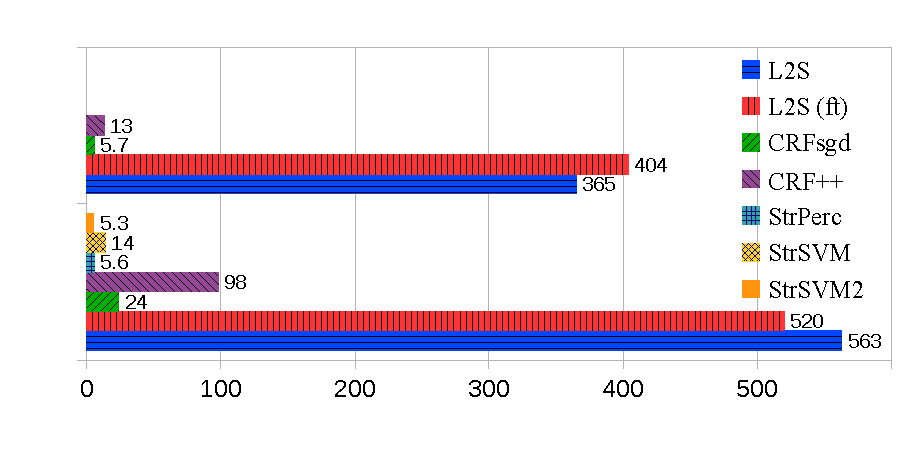
\includegraphics[scale=0.6]{../tokenposec.pdf}
    \caption{ICML 2015 Tutorial -- Hal Daum\'e III and John Langford }
  \end{figure}
\end{frame}

\subsection{Ulazni podaci}

\lstset{literate={ć}{{\'{c}}}1}

\defverbatim[colored]\lstV{
\begin{lstlisting}[basicstyle=\tiny\ttfamily]
2 |w Proces proces 0:6 ulllll
2 |w privatizacije privatizacije 0:13 lllllllllllll
1 |w na na 0:2 ll
2 |w Kosovu kosovu 0:6 ulllll
1 |w pod pod 0:3 lll
2 |w povećalom povećalom 0:9 lllllllll
\end{lstlisting}
}

\defverbatim[colored]\lstD{
\begin{lstlisting}[basicstyle=\tiny\ttfamily]
6 1 |w Proces |p NOUN  NOUNCase=Nom NOUNGender=Masc NOUNNumber=Sing
1 2 |w privatizacije |p NOUN  NOUNCase=Gen NOUNGender=Fem NOUNNumber=Sing
4 3 |w na |p ADP  ADPCase=Loc
6 2 |w Kosovu |p PROPN  PROPNCase=Loc PROPNGender=Neut PROPNNumber=Sing
6 3 |w pod |p ADP  ADPCase=Ins
0 4 |w povećalom |p NOUN  NOUNCase=Ins NOUNGender=Neut NOUNNumber=Sing
\end{lstlisting}
}

\begin{frame}{Ulaz u VW}{Označavanje vrste riječi}
  \lstV
\end{frame}

\begin{frame}{Ulaz u VW}{Ovisnosno parsanje}
  \lstD
\end{frame}

\subsection{Rezultati}

\begin{frame}{Rezultati}{POS}
  \begin{table}
  \centering
  \caption[Rezultat označavanja vrste riječi.]{Rezultat označavanja vrste riječi.
  Koristi se mjera točnosti.}
  \label{table:postagging}
  \begin{tabular}{|l|c|c|}
  \hline
  Metoda                               & \textsc{Set}   & \textsc{Wiki}  \\ \hline \hline
  HunPos (Agić et al., 2013)           & 97.04          & 94.62          \\
  \textsc{Vwpos-1}                     & 98.18          & 96.20          \\
  \textsc{Vwpos-2}                     & \textbf{98.71} & 96.24          \\
  \textsc{Vwmsd-1}                     & 98.31          & \textbf{96.57} \\
  \textsc{Vwmsd-2}                     & 98.23          & 96.41          \\ \hline
  \end{tabular}
  \end{table}
\end{frame}

\begin{frame}{Rezultati}{MSD}
  \begin{table}
  \centering
  \caption[Rezultat označavanja vrste riječi koristeći morfosintaktičke
  deskriptore.]{Rezultat označavanja vrste riječi koristeći morfosintaktičke
  deskriptore. Prikazana je točnost modela na dva testna skupa.}
  \label{table:msdtagging}
  \begin{tabular}{|l|c|c|}
  \hline
  Metoda                               & \textsc{Set}   & \textsc{Wiki}  \\ \hline \hline
  HunPos (Agić et al., 2013)           & 87.11          & 80.83          \\
  \textsc{Vwpos-1}                     & 89.94          & 83.27          \\
  \textsc{Vwpos-2}                     & \textbf{90.22} & \textbf{84.13} \\
  \textsc{Vwmsd-1}                     & 89.19          & 82.22          \\
  \textsc{Vwmsd-2}                     & 89.06          & 81.90          \\ \hline
  \end{tabular}
  \end{table}
\end{frame}

\begin{frame}{Rezultati}{Ovisnosno parsanje}
\begin{table}
\centering
\caption{Rezultat ovisnosnog parsanja.}
\label{table:depparsing}
\begin{tabular}{|l|c|c|}
\hline
Metoda                                & \textsc{las}   & \textsc{uas}    \\ \hline \hline
MSTParser (POS) (Agić i Merkler, 2013) & 74.56          & 81.59           \\
MSTParser (MSD) (Agić i Merkler, 2013) & 77.49          & 83.58           \\
\textsc{Vwdep} (POS)                  & 74.91          & 83.17           \\
\textsc{Vwdep} (MSD)                  & \textbf{79.22} & \textbf{86.44}  \\ \hline
\end{tabular}
\end{table}
\end{frame}

\begin{frame}{Rezultati}{Združeno označavanje vrste riječi i ovisnosno parsanje}
  \begin{table}
  \centering
  \caption[Rezultat označavanja vrste riječi sa združenim modelom.]{Rezultat
  označavanja vrste riječi sa združenim modelom. Prikazana je točnost modela na
  dva testna skupa.}
  \label{table:taggingjoint}
  \begin{tabular}{|l|l|l|l|l|}
  \hline
  Metoda           & \textsc{\textunderscript{Set}{pos}} & \textsc{\textunderscript{Wiki}{pos}} & \textsc{\textunderscript{Set}{msd}} & \textsc{\textunderscript{Wiki}{msd}} \\ \hline \hline
  \textsc{Vwpos-2} & \textbf{98.71}                      & 96.24                                & 90.22                               & 84.13                 \\
  \textsc{Vwjoint} & 98.69                               & \textbf{97.23}                       & \textbf{92.03}                      & \textbf{85.01}        \\ \hline
  \end{tabular}
  \end{table}
  \begin{table}
  \centering
  \caption{Rezultat ovisnosnog parsanja združenog modela.}
  \label{table:depparsing:joint}
  \begin{tabular}{|l|c|c|}
  \hline
  Metoda                 & \textsc{las}   & \textsc{uas}    \\ \hline \hline
  \textsc{Vwdep}   (MSD) & 79.22          & 86.44           \\
  \textsc{Vwjoint} (POS) & 75.44          & 83.91           \\
  \textsc{Vwjoint} (MSD) & \textbf{81.01} & \textbf{88.02}  \\ \hline
  \end{tabular}
  \end{table}
\end{frame}

\appendix
\backupbegin

\begin{frame}{Dodatak}
\begin{itemize}
    \item dodatak
    \item dodatak
    \item dodatak
\end{itemize}
\end{frame}

\backupend

\end{document}
